\section{Lower Bounds for the Extension Complexity}
% todo: Think about multi-dimensional proof

In this section we provide yet another proof for $pc(n) \in \Omega(n^{1/2})$.

After the proof is done, we will explain the key concepts of the applied theorem and show how to apply it in general.

The central piece of the proof is Theorem~1 from \cite{averkov2016maximum}, which we adopt for the case of linear extended formulations (the original also allowed semidefinite ones).

Therefore we have to introduce the \textit{Hausdorff distance} of two non-empty compact sets $X,Y \subseteq \R^d$, which can be thought of "the longest distance you can be forced to travel from a point in one of the two sets to the other set". See Figure~\ref{fig:hausdorff} for an example.

\begin{figure}[h]
  \centering
  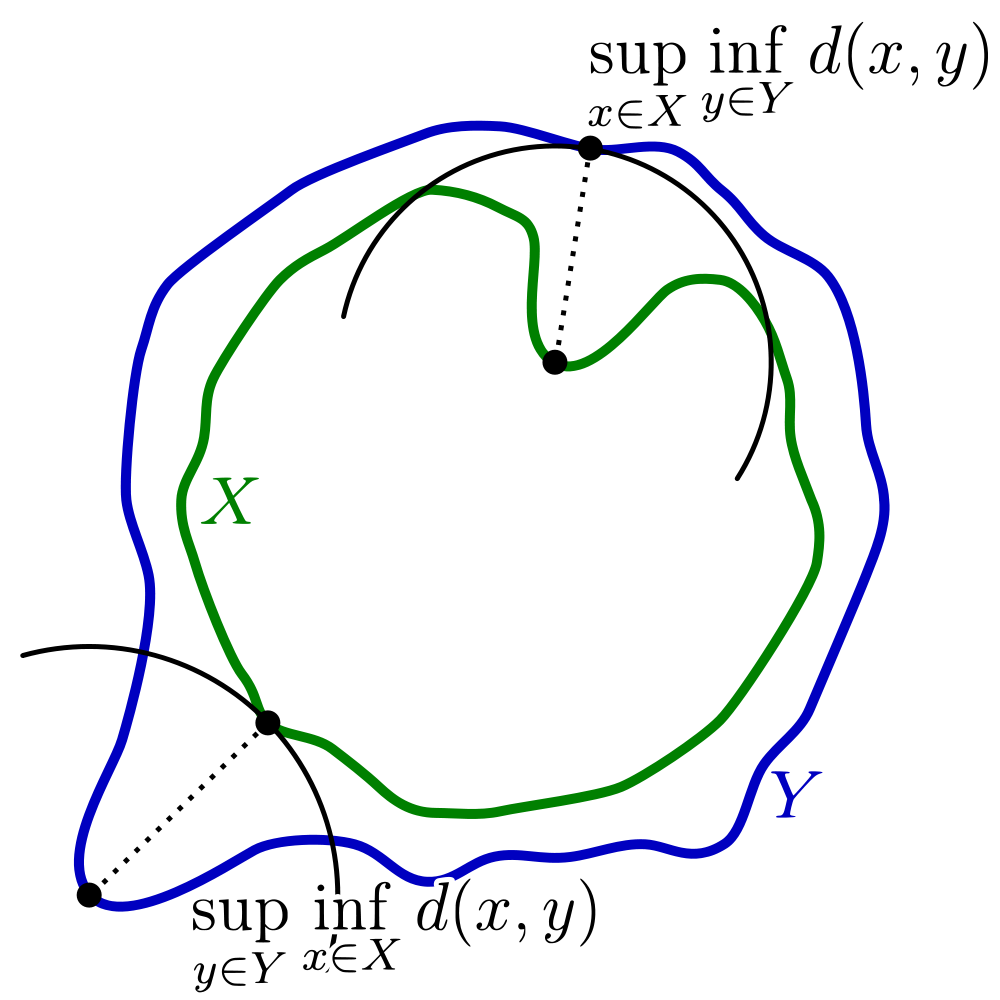
\includegraphics[height=55mm]{assets/Hausdorff_distance.png}
  \caption{Hausdorff distance example \cite{rocchini2007hausdorff}}
  \label{fig:hausdorff}
\end{figure}

\begin{definition}[Hausdorff distance]
  The \textit{Hausdorff distance} with respect to the Euclidean norm is defined by $$ \dist_H(X,Y) := \max \left\{ \sup_{x \in X} \inf_{y \in Y} \norm{x-y}, \sup_{y \in Y} \inf_{x \in X} \norm{x-y} \right\} .$$
\end{definition}

\begin{theorem}[{\cite[Theorem 1]{averkov2016maximum}}, adopted]\label{theorem:family}
  Let $\P$ be a family of polytopes in $\R^d$ of dimensions at least one with $2 \leq \abs{\P} < \infty $ such that each $P \in \P$ has an extended formulation of size $m$.
  Let $\rho > 0$ and $\Delta > 0$ be such that each $P \in \P$ is contained in the ball $\rho \B^d$ and, 
  for every two distinct polytopes $P \in \P$ and $P' \in \P$, one has $\dist_H(P, P') \geq \Delta$. 
  Then $$m^2 \geq \frac{\log_2 \abs{\P}}{8d \left(1 + \log_2 (2\rho/\Delta) + \log_2\log_2 \abs{\P} \right)} =: B.$$
  In particular, we have $$\max \{\xc(P) \mid P \in \P\}  \geq \sqrt{B} .$$
\end{theorem}



\subsection{Proof of Lower Bound}

\begin{corollary}
  $pc(n) \in \Omega(\sqrt{n})$
\end{corollary}
\begin{proof}
  To apply \ref{theorem:family} we have to pick a familiy of polytopes $\P$. Then we have to determine $\rho$ and $\Delta$ and bound $\log_2 \abs{\P}$ from below and $\log_2 \log_2 \abs{\P}$ from above.

  So we choose $n^2$ fixed points evenly on the unit circle (so they would form a regular polygon). Let $\P_n$ be the familiy of polygons, where each polygon has $n$ vertices chosen from the $n^2$ points on the unit circle.

  Then $\rho = 1$, since all polygons are contained in the unit circle.

  For two distinct polygons $P, P' \in \P_n$ one of them has a vertex $v$, which the other one does not have. W.l.o.g $v \notin P, v \in P'$. So $\dist_H(P,P') \geq \inf_{p \in P} \norm{v-p} \geq d_{min}$ (see Figure~\ref{fig:distance} for the definition of $d_{min}$).

  \begin{figure}[h]
    \centering
    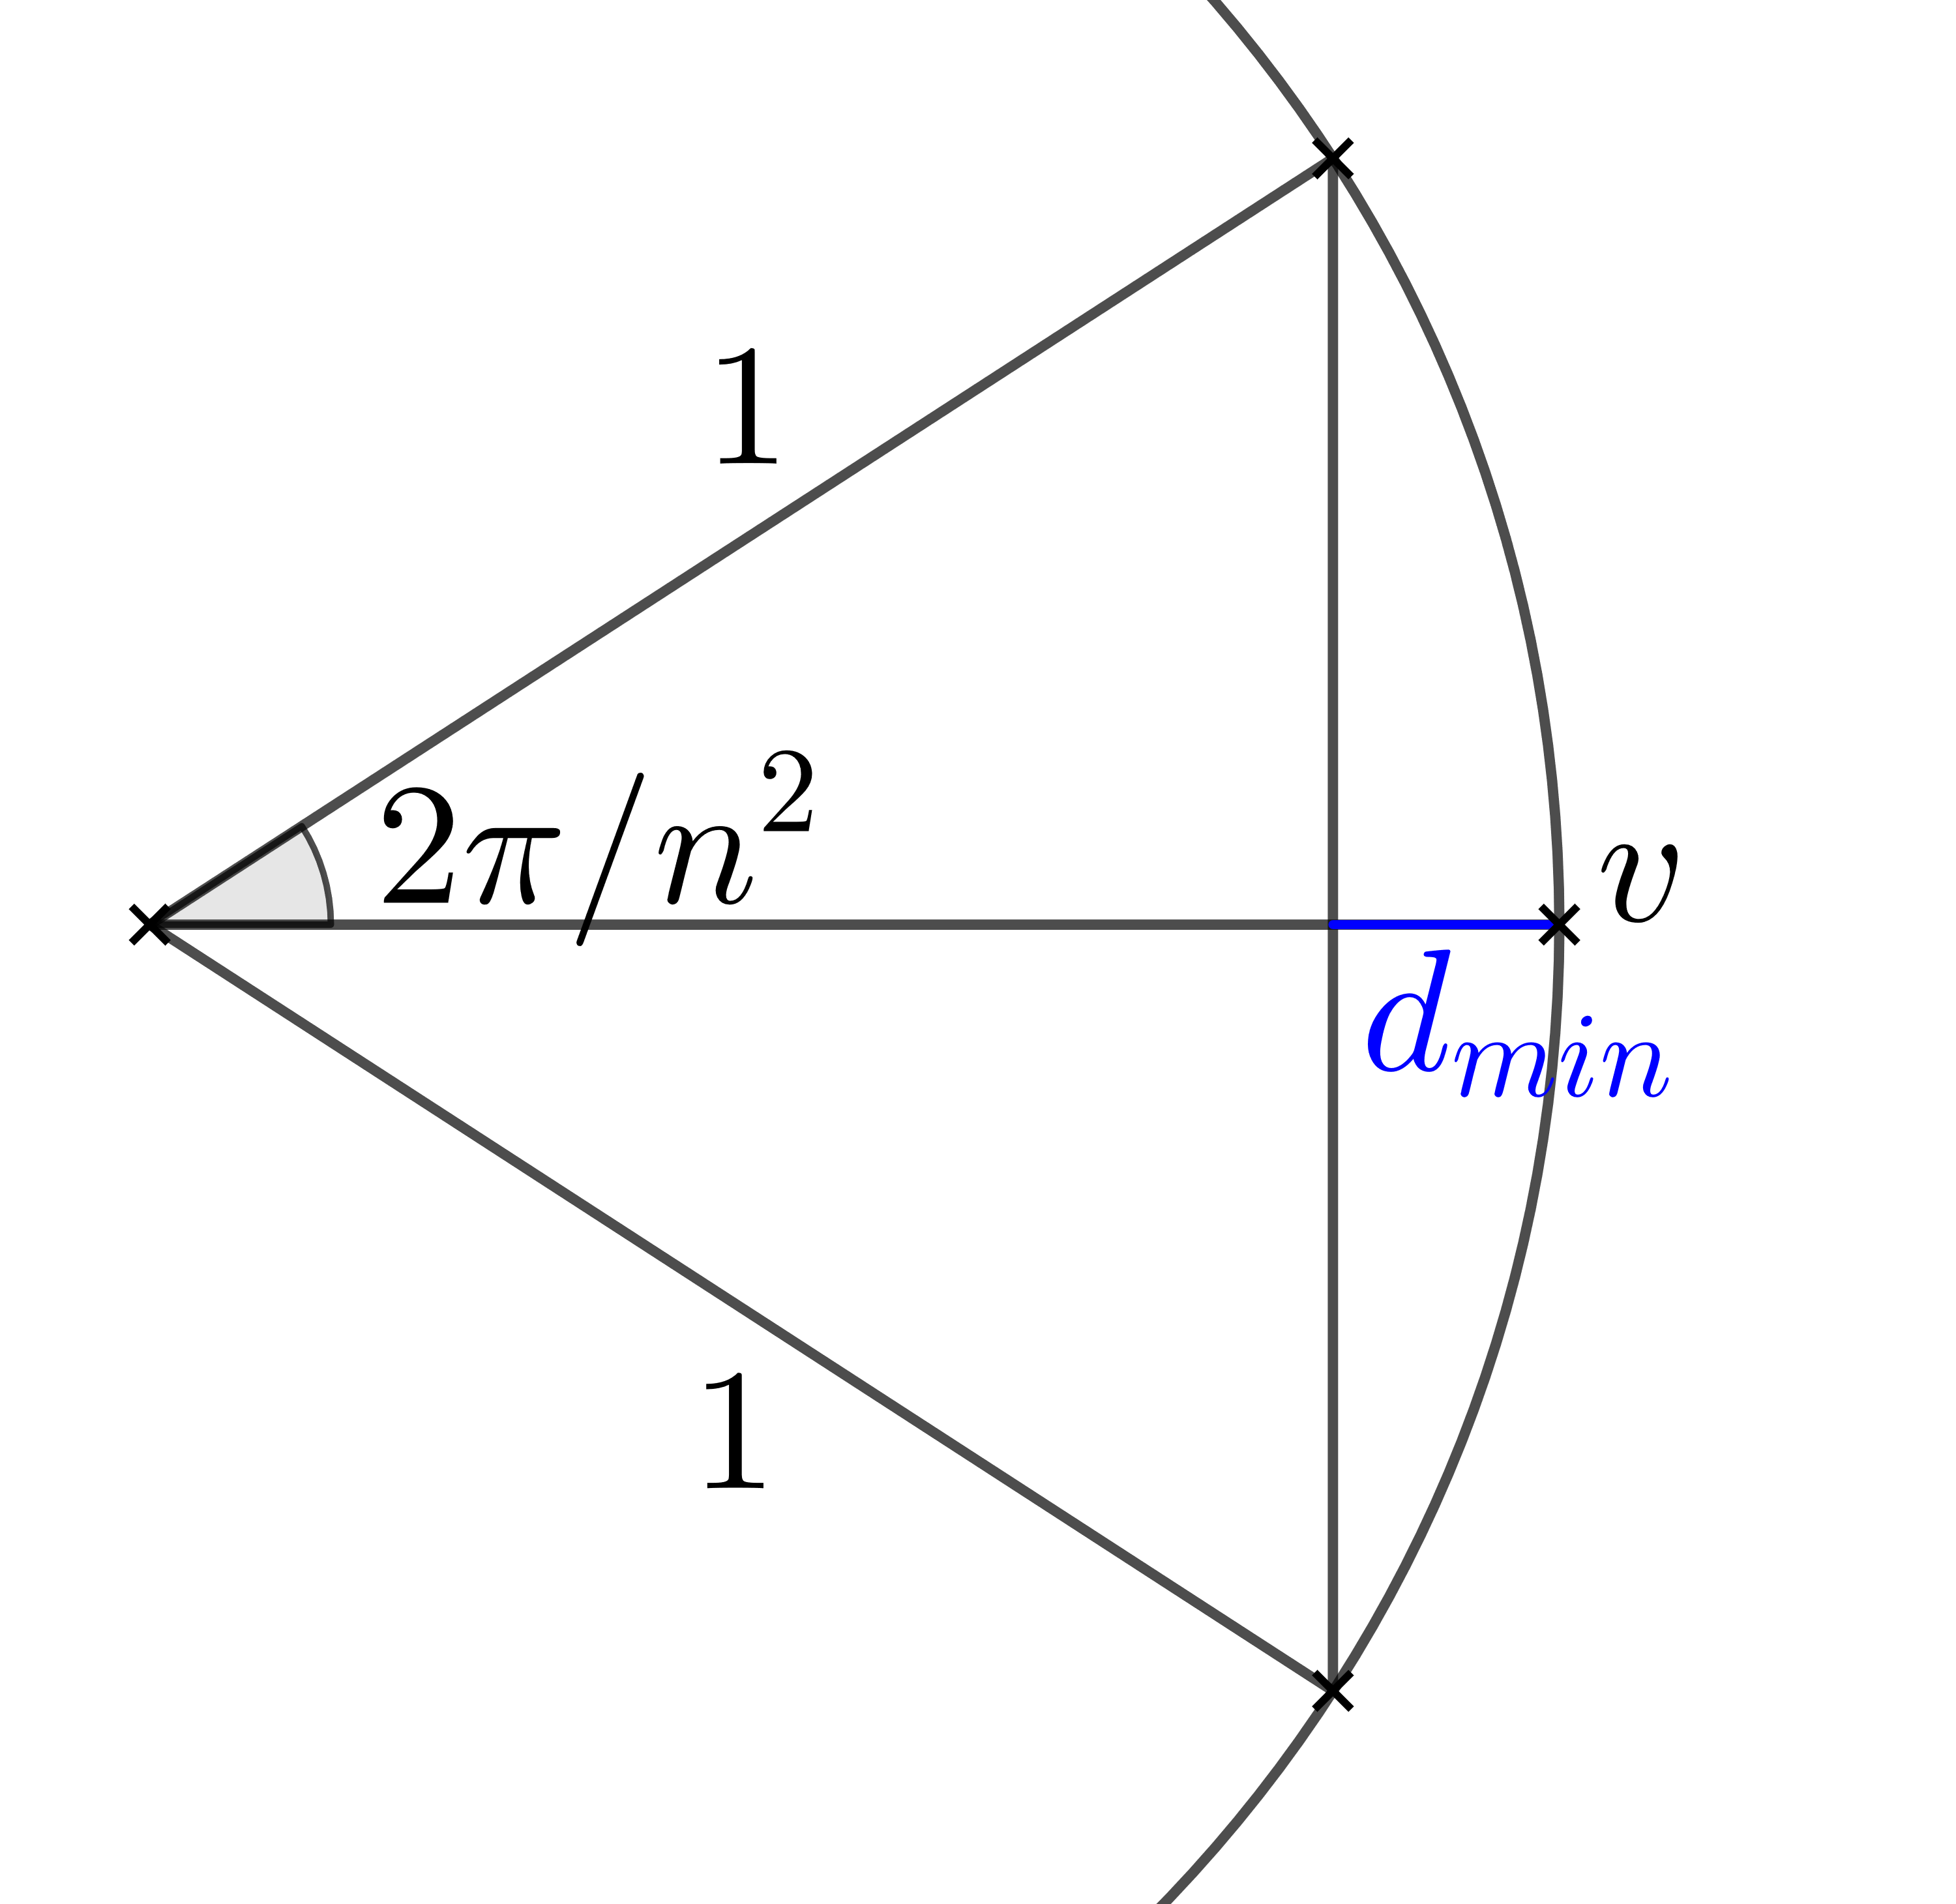
\includegraphics[height=55mm]{assets/Minimal_Hausdorff_distance.png}
    \caption{Definition of $d_{min}$}
    \label{fig:distance}
  \end{figure}
  
  \begin{align*}
    1 - d_{min} &= \cos\left( \frac{2 \pi}{n^2} \right)\\
    d_{min} &\geq 1 - \left(1 - \frac{\left(\frac{2 \pi}{n^2}\right)^2}{2} \right) = 2 \frac{\pi^2}{n^4} =: \Delta
  \end{align*}

  For the estimate we used $\cos(x) \leq 1 - \frac{x^2}{2!}$, which arises from the power series for cosine.

  Since each polygon in $\P_n$ is defined by $n$ points, chosen from a set of $n^2$ points, $\abs{\P_n} = \binom{n^2}{n}$. Therefore $n^n = \left( \frac{n^2}{n} \right)^n \leq \abs{\P_n} \leq \left( n^2 \right)^n = n^{2n}$. $\log_2 \abs{\P_n} \geq n \log_2 n$ and $\log_2 \log_2 \abs{\P_n} \leq \log_2 (2n \log_2 n) = 1 + \log_2 n + \log_2 \log_2 n$.

  Now we can calculate $B$ from Theorem~\ref{theorem:family}:
  \begin{align*}
    B &= \frac{\log_2 \abs{\P_n}}{8d \left(1 + \log_2 (2\rho/\Delta) + \log_2\log_2 \abs{\P_n} \right)}\\
    &\geq \frac{n \log_2 n}{16 \left(1 + \log_2 (n^4 / \pi^2) + 1 + \log_2 n + \log_2 \log_2 n \right)}\\
    &= \frac{n \log_2 n}{16 \left(2 - 2 \log_2 \pi + 5 \log_2 n + \log_2 \log_2 n \right)}\\
    &\geq \frac{n}{16*6}
  \end{align*}

  For the last inequality we used $2 - 2 \log_2 \pi \leq 0$ and $\frac{5 \log_2 n + \log_2 \log_2 n}{\log_2 n} \leq 6$ for $n \geq 1$.

  Therefore we can conclude $$\pc(n) \geq \max \{\xc(P) \mid P \in \P_n\} \stackrel{\text{(Th. \ref{theorem:family})}}{\geq} \sqrt{B} \geq \frac{1}{12} \sqrt{n} .$$
\end{proof}



\subsection{Key Ideas Behind the Applied Theorem}
% todo: formulate

\begin{enumerate}
  \item Encode polytopes trough normalized extended formulations (Everything from now on in encoding vector space)
  \item Bound pairwise distance from below (using $\Delta$)
  \item Draw spheres around enconding point (half of min distance)
  \item Bound radius of containing ball from above (using $\rho$)
  \item Bound maximum number of possible by volume (how many encodings can fit in containing ball)
\end{enumerate}
